
\documentclass[./Thick_TQFTs_and_Quantum_Information.tex]{subfiles}

\begin{document}

\section{Paths for Parallel Transport}

In order to obtain linear maps by parallel transport on manifolds, we need
additional structure on top of connections. These are collections of paths on
manifolds along which we will parallel transport vectors in the fibres of a
bundle with connection. We shall now formalize this apparatus in terms of
categories. We will require a notion of graphs on manifolds whose vertices are
points, possibly repeated, on the manifold and whose edges are paths on the
manifold.

\subsection{Graphs Encoding Algebraic Expressions}

We will now define a class of graphs that encode expressions involving tensor
products, point-wise algebra products and composition of linear maps $A \to A$
for some algebra $A$. As a matter of convention, we will take all graphs to mean
multidigraphs -- directed graphs where we allow parallel edges including
self-loops. Given a graph $G = (V, E)$, we will write $V = V(G)$ and $E(G)$, and
will denote the set of edges from a vertex $u$ to a vertex $v$ in $G$ as
$G(u, v)$.

\begin{defn}[Elementary Expression Graph]\label{eeg}
Let $G = (V, E)$ be a finite graph satisfying the following properties:
\begin{enumerate}[(i)]

\setlength{\itemsep}{0pt}

\item \label{eeg:part}
$V = V_1 \amalg \dots \amalg V_k$ for some $k \in \N \cup \set{0}$, with each
$V_i$ totally ordered as $V_i = \set{v_{i, 1}, \dots, v_{i, q_i}}$ for some
$q_i \in \N$

\item \label{eeg:loop}
each vertex $v \in V$ has exactly one self-loop

\item \label{eeg:forward}
for every edge from $u$ to $v$ in $E$ that is not a self-loop, $u \in V_i$ and
$v \in V_{i + 1}$ for some $i \in \set{1, \dots, k - 1}$, when $k \geq 2$

\item \label{eeg:nonredright}
each point in $V_{i + 1}$ has at least one edge from a point in $V_{i}$,
$1 \leq i < k$

\item \label{eeg:nonredleft}
each point in $V_{i}$ has at least one edge to a point in $V_{i + 1}$,
$1 \leq i < k$

\end{enumerate}
Then $G$ is called an elementary expression graph and for any vertex $v \in V$,
we write $p_{G}(v)$ to denote the number $i$ for which $v \in V_i$.
\end{defn}

\begin{rmk}
The total ordering on vertex set parts in condition \eqref{eeg:part} is needed
for defining a ``composition'' or gluing of expression graphs later on.
\end{rmk}

\begin{rmk}
Property \eqref{eeg:forward} above guarantees that $V_1$ has no incoming edges,
$V_k$ has no outgoing edges and, except for self-loops, there are no edges
``going backwards'' or ``staying within parts'' -- that is, from $V_j$ to $V_i$
for $i \leq j$. It also guarantees that there are no edges ``skipping the next
part'' -- that is, from $V_i$ to $V_j$ for $j > i + 1$.
\end{rmk}

\begin{exm}\label{exm:egraph1}
Consider the graph consisting of nine vertices $1, \dots, 9$ with
$V_1 = \set{1, 2}$, $V_2 = \set{3, 4}$, $V_4 = \set{5, 6, 7}$ and
$V_4 = \set{8, 9}$, along with edges (without listing self-loops):
\[\begin{array}{ccccc}
  (1, 3) &,& (1, 4) &,& (2, 3),\\
  (3, 5) &,& (3, 6) &,& (4, 7),\\
  (5, 8) &,& (6, 9) &,& (7, 9)
\end{array}\]
It is easy to check that this graph satisfies all conditions in the definition
of an elementary expression graph by visualizing it as follows, skipping
self-loops:
\[\begin{tikzpicture}[baseline=(a).base]
\node[scale=\diagscale] (a) at (0, 0){
\begin{tikzcd}[column sep=huge, row sep=tiny]
                  &                   & 5 \ar[rd] &   \\
1 \ar[r] \ar[rdd] & 3 \ar[ru] \ar[rd] &           & 8 \\
                  &                   & 6 \ar[rd] &   \\
2 \ar[ruu]        & 4 \ar[rd]         &           & 9 \\
                  &                   & 7 \ar[ur] &
\end{tikzcd}
};
\end{tikzpicture}\]

We then observe that we can use this graph to generate an algebraic expression
of the form:
\[
  ((5, 8) \tensor ((6, 9) \cdot (7, 9))) \circ
  ((3, 5) \tensor (3, 6) \tensor (4, 7)) \circ
  (((1, 3) \cdot (2, 3)) \tensor (1, 4))
\]
where the rule is roughly as follows: we infix $(6, 9)$ and $(7, 9)$ with
`$\cdot$' because they share the same target vertex and we call $9$ the target
vertex of $(6, 9) \cdot (7, 9)$; we infix the expressions $(6, 9) \cdot (7, 9)$
and $(5, 8)$ with a `$\tensor$' because they do not share the same target vertex
and we call the expression $5 \tensor 6 \tensor 7$ the source and the expression
$8 \tensor 9$ the target of the expression
$(5, 8) \tensor ((6, 9) \cdot (7, 9))$. For expressions $E_1$ and $E_2$ such
that the target of $E_1$ is the source of $E_2$, we call these expressions
composeable and we form the new expression $E_2 \circ E_1$. This yields the
whole expression above.

One sees readily the edges can be replaced with paths in a manifold $M$ equipped
with an $A$--fibred bundle with connection. These paths can then be replaced
replaced with linear maps $A \to A$ yielding a linear map corresponding to the
expression. We can associate this linear map to $M$ in some notion of TQFT. This
will later motivate us to define an algorithm for obtaining a canonical
expression from an expression graph.
\end{exm}

We observe that we can take disjoint unions of elementary expression graphs but
the result is not an \textit{elementary} expression graph, in general, because
the pieces of the disjoint union do not all have the same number of parts. For
this, we define the following.

\begin{defn}[Expression Graph]
A disjoint union of elementary expression graphs
$G = G_1 \amalg \dots \amalg G_n$ is called an expression graph. We have a part
function for each component expression graph -- that is, $p_{G_i}(u) = j$ if and
only if $u \in G_i$, the vertex set of $G_i$ is $\coprod_{j = 1}^{k_i} V_{i, j}$
and $u \in V_{i, j}$ for some $j$.
\end{defn}

In order to obtain a category of expression graphs with monoidal structure given
by disjoint union, we define morphisms of expression graphs. For this, we first
define a homomorphism of (multidi-)graphs suitable for our purposes.

\begin{defn}[Multidigraph Homomorphism]
For multidigraphs $G$ and $H$, a function $h : V(G) \to V(H)$ along with
functions $h_{u, v} : G(u, v) \to H(h(u), h(v))$, for every $u, v \in V(G)$,
is called a multidigraph homormophism or simply a graph homomorphism. We will
write the multidigraph homomorphism -- that is, the pair
$(h, \set[h_{u, v}]{u, v \in V(G)})$ -- as simply $h : G \to H$ and we will
write $h(u)$ for vertices $u$ as well as $h(e)$ for edges $e$ when the endpoints
of $e$ are not important. If $G'$ is a subgraph of $G$, we will write the
subgraph of $H$ formed by $h(V(G'))$ and $h_{u, v}(G'(u, v))$ for all
$u, v \in V(G')$ as $h(G')$.
\end{defn}

\begin{defn}[Expression Homomorphism]
For $i = 1, \dots, n$ and $j = 1, \dots, m$, let
\[
  G_i = \br{\coprod_{k = 1}^{p_i} V_{G_i, k}, E_{G_i}} \text{ and }
  H_j = \br{\coprod_{k = 1}^{q_i} V_{H_j, k}, E_{H_j}}
\]
be elementary expression graphs such that $G = \coprod_{i} G_i$ and
$H = \coprod_{j} H_j$ are expression graphs. Then, an expression homomorphism is
a graph homomorphism $h : G \to H$ satisfying the following:
\begin{enumerate}[(i)]

\item for all $i = 1, \dots, n$, $h(G_i) \subset H_j$ for some
$j \in \set{1, \dots, m}$

\item for all $i, j, k, k'$, $h|_{V_{G_i, k}} : V_{G_i, k} \to V_{H_j, k'}$ is
monotone or order-preserving

\item for vertices $u, v \in V(G_i)$ with $h(u), h(v) \in V(H_j)$,
\[
  p_{G_i}(u) = p_{G_i}(v) \iff p_{H_j}(h(u)) = p_{H_j}(h(v))
\]
\end{enumerate}
\end{defn}

\begin{rmk}
The conditions in the definition above ensures that $h$ restricted to each
elementary expression graph in its domain is also a homomorphism into an
elementary expression graph in the codomain.
\end{rmk}

It is easy to see that expression graphs with expression homomorphisms form a
category with monoidal structure given by disjoint union as the monoidal product
and the empty expression graph as the monoidal unit. The associators and unitors
transfer over from the category of sets and are easily verified to be transport
homomorphisms. The associators and unitors satisfy the coherence axioms since
they do so in the category of sets. \TODO{Add an appendix entry for this.}

\begin{defn}[Category of Expression Graphs]
We call this monoidal category the category of expression graphs and denote it
$\EG$. We denote the maximal subgroupoid of $\EG$ as $\EG^{\text{iso}}$
\end{defn}

\begin{defn}[Category of Single Part Expression Graphs]
The subcategory of $\EG$ consisting of expression graphs with only one vertex
part is called the category of single part expression graphs and denote $\EG_1$.
We denote the maximal subgroupoid of $\EG_1$ as $\EG_1^{\text{iso}}$.
\end{defn}

\begin{rmk}
The isomorphisms in $\EG_1$ are unique because they are monotone bijections
between finite sets of equal size.
\end{rmk}

We will now define a notion of gluing for expression graphs. To this end, we
define the ``source'' and ``target'' ends of an expression graph in the obvious
way.

\begin{defn}[Source and Target of an Expression Graph]
Let $G = \coprod_{i = 1}^{n} G_i$ be an expression graph in a manifold $M$ with
$G_i$ having the vertex partition $\coprod_{j = 1}^{k_i} V_{i, j}$. Then, we
define the source of $G$ as the expression graph $S(G)$ with vertex set
$\coprod_{i = 1}^{n} V_{i, 1}$ consisting of a single part and and edge set
consisting of only self-loops. The target
of $G$ is the expression graph $T(G)$ defined analogously with the vertex set
$\coprod_{i = 1}^{n} V_{i, k_i}$.
\end{defn}

\begin{rmk}
We notice that the total ordering of vertex set parts of each elementary
expression graph in an expression graph along with the ordering of the elementary
expression graphs themselves induces a total ordering of $S(G)$ and $T(G)$,
respectively. At the same time, there are unique inclusion expression
homomorphisms
\[
  S(G) \hto[s_G] G \hot[t_G] T(G)
\]
\end{rmk}

\begin{lem}
Let $G$ and $H$ be expression graphs such that $|S(H)| = |T(G)|$.
We then have a unique expression homomorphism $\psi_{G, H} : T(G) \to S(H)$ which
is monotone on vertex sets. The pushout in $\EG$ of the follosing diagram
exists:
\[
  G \hot[t_G] T(G) \to[\psi_{G, H}] S(H) \hto[s_H] H
\]
\end{lem}
\begin{proof}
We consider the pushout of the diagram in $\Set$ for both the vertex and edge
sets. Then it is easy to see that the resulting vertex and edge sets satisfy the
conditions of the definition of an expression graph -- we are simply identifying
the isomorphic subgraphs $S(H)$ of $H$ and $T(G)$ of $G$ in the disjoint union
$G \amalg H$.
\end{proof}

\begin{defn}[Gluing Expression Graphs]
We define the pushout above to be the gluing $H * G = G \amalg_{S(H)} H$ in
$\EG$. If $G$ and $H$ satisfy the condition $|S(H)| = |T(G)|$ as above, we call
them gluable at $S(H) \cong T(G)$.
\end{defn}

Taking $S(G)$ and $T(G)$ as the identities of $G$ for this gluing operation, it
is straightforward to verify that the associators and unitors for pushouts in
the category of sets are expression homomorphisms. Hence, these associators and
unitors also satisfy associativity and unity coherence axioms to make the
following theorem true. \TODO{Add and appendix entry for the proof of this.}

\begin{thm}
The following data form a monoidal double category:
\begin{enumerate}[(i)]
\setlength{\itemsep}{0pt}
\item Object Category: $\EG_1^{\text{iso}}$
\item Morphism Category: $\EG^{\text{iso}}$
%\item $2$--morphisms: for horizontal $1$--morphisms $G$ and $H$ with isomorphic
%source and targets, expression homomorphisms  making the
%following diagram commute (with the obvious inclusions):
%\[
%\begin{tikzpicture}[baseline=(a).base]
%\node[scale=\diagscale] (a) at (0, 0){
%\begin{tikzcd}
%               & S(G) \cong S(H) \ar[ld, hook] \ar[rd, hook] &   \\
%G \ar[rr, "f"] &                                             & H \\
%               & T(G) \cong T(H) \ar[ul, hook] \ar[ur, hook] &
%\end{tikzcd}
%};
%\end{tikzpicture}
%\]
\item Source and Target Functors: $S : G \mapsto S(G)$ and $T : G \mapsto T(G)$
with the obvious action on $2$--morphisms -- each $2$--morphism maps to a unique
isomorphism in the object category
\item Unit Functors: $S$ (left) and $T$ (right)
\item Horizontal Composition Associators: pushout associators inherited from
$\Set$
\item Horizontal Composition Unitors: pushout unitors inherited from $\Set$
\item Monoidal Product: disjoint union
\item Monoidal Unit: empty expression graph
\end{enumerate}
\end{thm}

\begin{defn}[Double Category of Expression Graphs]
The double category of the above theorem is called the double category of
expression graphs and is denoted $\DEG$
\end{defn}

\begin{rmk}
We could instead show that $\EG$ has all pushouts so that the above double
category is merely a sub-category of the double category of cospans in $\EG$. In
fact, I think this is how we should prove it in the appendix if we do.
\end{rmk}

\subsection{Geometric Realization}

We wish to use expression graphs to generate linear maps by viewing the edges as
paths in a manifold equipped with an algebra-fibred bundle with connection,
taking their associated parallel transport maps, and combining these maps in a
pattern encoded in the expression graph. To accomplish this, we use the
following simple notion of geometric realization of graphs.

\begin{defn}[Geometric Graph]
A graph in a manifold $M$ or a geometric graph is a graph $G = (V, E)$ equipped
with a function $\gamma : E \to C^0(I, M)$, called a geometric realization of
$G$. We call $M$ the realizing manifold of $G$ under $\gamma$.

For an edge from $u$ to $v$ we write $\gamma_{u, v}$ to denote the path
associated to that edge when no parallel edges from $u$ to $v$ exist. If there
are two edges from $u$ to $v$ with labels $e_1$ and $e_2$, then we write
$\gamma_{e_1}$ and $\gamma_{e_2}$ to denote the paths associated to $e_1$ and
$e_2$, respectively.
\end{defn}

\begin{rmk}
A geometric graph is essentially a collection of paths in a manifold but we
consider one or more copies of each path and ``identify'' their end-points in a
pattern encoded by a graph, even though these paths need not share end-points --
that is, we do not strictly require $\gamma_{u, v}(1) = \gamma_{v, w}(0)$. We
will see that this relaxation is essential to defining our notion of TQFTs. We
will ultimately be interested in expression graphs in manifolds, which will
provide us with a way to associate linear maps to manifolds.
\end{rmk}

\begin{defn}[Geometric Homomorphism]
Let $G$ and $H$ be graphs in manifolds $M$ and $N$ with geometric realizations
$\gamma^G$ and $\gamma^H$ respectively, then a homomorphism $h : G \to H$
equipped with a smooth map $f : M \to N$ making the following diagram commute is
called a geometric homomorphism:
\[
\begin{tikzpicture}[baseline=(a).base]
\node[scale=\diagscale] (a) at (0, 0){
\begin{tikzcd}
E(G) \ar[d, "\gamma^G" left] \ar[r, "h" above] &
E(H) \ar[d, "\gamma^H" right] \\
C^0(I, M) \ar[r, "f_*" below] &
C^0(I, N)
\end{tikzcd}
};
\end{tikzpicture}
\]
where $f_*$ is the post-composition map $g \mapsto f \circ g$.
\end{defn}

Pasting commutative squares as the one above along the $\gamma$ sides, we
observe that geometric homomorphisms compose associatively. Taking
$h$ and $f$ as the identity maps yields an identity morphism of geometric
graphs. It is also straightforward to verify that disjoint union gives
geometric graphs along with geometric homomorphisms a monoidal structure with
the empty graph in the empty manifold as the monoidal unit.
\TODO{Add an appendix entry for this.}

\begin{defn}[Categories of Geometric Graphs]
We denote the monoidal category of geometric graphs and geometric
homomorphisms as $\textbf{Graph}_{\Man}$. The subcategory of
$\textbf{Graph}_{\Man}$ consiting of geometric expression graphs and geometric
expression homomorphisms is denoted $\EG_{\Man}$. The subcategory of
$\EG_{\Man}$ obtained by considering geometric expression graphs in manifolds
within a subcategory $\s{C}$ of $\Man$ is denoted $\EG_{\s{C}}$.
\end{defn}

\begin{exm}
If $\Diff_d$ is the subcategory of $\Man$ consisting of $d$--dimensional
manifolds and diffeomorphisms only, then $\EG_{\Diff_d}$ is the corresponding
subcategory of $\EG_{\Man}$.
\end{exm}

\begin{exm}
Let $\Man(M)$ be the subcategory of $\Man$ consisting of a manifold $M$ and all
smooth maps $M \to M$. $\EG_{\Man(M)}$ is the corresponding subcategory of
$\EG_{\Man}$. In this case, we also denote this subcategory as $\EG_M$.
\end{exm}

\begin{exm}
Consider the graph in example \ref{exm:egraph1}. Then, we consider a mapping of
the edges to paths on a surface as shown below.\footnote{This diagram was
generated using \cite{Mathcha}.} We do not show the paths associated to
self-loops. Note that here we have $\gamma_{u, v}(1) = \gamma_{v, w}(0)$ for
most points but not all -- for instance, $\gamma_{2, 3}$ and $\gamma_{3, 5}$ do
not share any end-points.
\begin{figure}[H]
\begin{center}

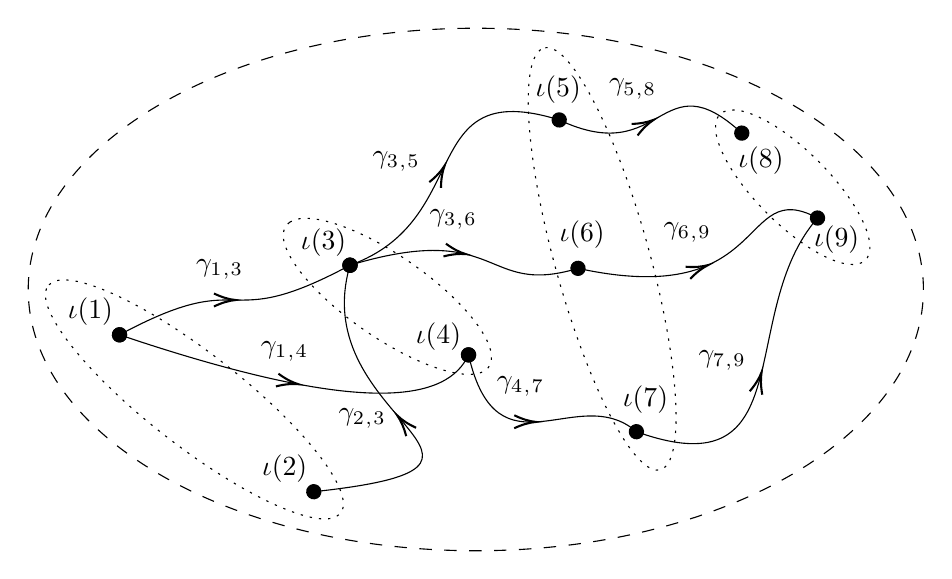
\begin{tikzpicture}[x=0.75pt,y=0.75pt,yscale=-0.95,xscale=0.95]
%uncomment if require: \path (0,281); %set diagram left start at 0, and has height of 281

%Shape: Ellipse [id:dp45216116111361904] 
\draw  [dash pattern={on 4.5pt off 4.5pt}] (6,138.5) .. controls (6,65.32) and (107.63,6) .. (233,6) .. controls (358.37,6) and (460,65.32) .. (460,138.5) .. controls (460,211.68) and (358.37,271) .. (233,271) .. controls (107.63,271) and (6,211.68) .. (6,138.5) -- cycle ;
%Curve Lines [id:da12378300176275903] 
\draw    (52.31,161.49) .. controls (119.1,125.59) and (102.4,162.09) .. (169.19,126.19) ;
\draw [shift={(169.19,126.19)}, rotate = 331.74] [color={rgb, 255:red, 0; green, 0; blue, 0 }  ][fill={rgb, 255:red, 0; green, 0; blue, 0 }  ][line width=0.75]      (0, 0) circle [x radius= 3.35, y radius= 3.35]   ;
\draw [shift={(111.13,143.84)}, rotate = 180.1] [color={rgb, 255:red, 0; green, 0; blue, 0 }  ][line width=0.75]    (10.93,-3.29) .. controls (6.95,-1.4) and (3.31,-0.3) .. (0,0) .. controls (3.31,0.3) and (6.95,1.4) .. (10.93,3.29)   ;
\draw [shift={(52.31,161.49)}, rotate = 331.74] [color={rgb, 255:red, 0; green, 0; blue, 0 }  ][fill={rgb, 255:red, 0; green, 0; blue, 0 }  ][line width=0.75]      (0, 0) circle [x radius= 3.35, y radius= 3.35]   ;
%Curve Lines [id:da3902364739215902] 
\draw    (169.19,126.19) .. controls (233.04,103.33) and (202.45,29.92) .. (275.29,52.51) ;
\draw [shift={(275.29,52.51)}, rotate = 17.23] [color={rgb, 255:red, 0; green, 0; blue, 0 }  ][fill={rgb, 255:red, 0; green, 0; blue, 0 }  ][line width=0.75]      (0, 0) circle [x radius= 3.35, y radius= 3.35]   ;
\draw [shift={(217.18,75.67)}, rotate = 476.11] [color={rgb, 255:red, 0; green, 0; blue, 0 }  ][line width=0.75]    (10.93,-3.29) .. controls (6.95,-1.4) and (3.31,-0.3) .. (0,0) .. controls (3.31,0.3) and (6.95,1.4) .. (10.93,3.29)   ;
\draw [shift={(169.19,126.19)}, rotate = 340.3] [color={rgb, 255:red, 0; green, 0; blue, 0 }  ][fill={rgb, 255:red, 0; green, 0; blue, 0 }  ][line width=0.75]      (0, 0) circle [x radius= 3.35, y radius= 3.35]   ;
%Curve Lines [id:da5125133831866234] 
\draw    (52.31,161.49) .. controls (178.45,204.05) and (218.84,194.46) .. (229.3,171.66) ;
\draw [shift={(229.3,171.66)}, rotate = 294.65] [color={rgb, 255:red, 0; green, 0; blue, 0 }  ][fill={rgb, 255:red, 0; green, 0; blue, 0 }  ][line width=0.75]      (0, 0) circle [x radius= 3.35, y radius= 3.35]   ;
\draw [shift={(142.99,186.54)}, rotate = 191.16] [color={rgb, 255:red, 0; green, 0; blue, 0 }  ][line width=0.75]    (10.93,-3.29) .. controls (6.95,-1.4) and (3.31,-0.3) .. (0,0) .. controls (3.31,0.3) and (6.95,1.4) .. (10.93,3.29)   ;
\draw [shift={(52.31,161.49)}, rotate = 18.65] [color={rgb, 255:red, 0; green, 0; blue, 0 }  ][fill={rgb, 255:red, 0; green, 0; blue, 0 }  ][line width=0.75]      (0, 0) circle [x radius= 3.35, y radius= 3.35]   ;
%Curve Lines [id:da9936282267570157] 
\draw    (150.83,241.06) .. controls (275.76,227.54) and (145.96,205.62) .. (169.19,126.19) ;
\draw [shift={(169.19,126.19)}, rotate = 286.3] [color={rgb, 255:red, 0; green, 0; blue, 0 }  ][fill={rgb, 255:red, 0; green, 0; blue, 0 }  ][line width=0.75]      (0, 0) circle [x radius= 3.35, y radius= 3.35]   ;
\draw [shift={(193.16,202.39)}, rotate = 409.89] [color={rgb, 255:red, 0; green, 0; blue, 0 }  ][line width=0.75]    (10.93,-3.29) .. controls (6.95,-1.4) and (3.31,-0.3) .. (0,0) .. controls (3.31,0.3) and (6.95,1.4) .. (10.93,3.29)   ;
\draw [shift={(150.83,241.06)}, rotate = 353.83] [color={rgb, 255:red, 0; green, 0; blue, 0 }  ][fill={rgb, 255:red, 0; green, 0; blue, 0 }  ][line width=0.75]      (0, 0) circle [x radius= 3.35, y radius= 3.35]   ;
%Curve Lines [id:da37329721640419344] 
\draw    (229.3,171.66) .. controls (243.97,235.64) and (284.76,184.82) .. (314.44,210.62) ;
\draw [shift={(314.44,210.62)}, rotate = 41] [color={rgb, 255:red, 0; green, 0; blue, 0 }  ][fill={rgb, 255:red, 0; green, 0; blue, 0 }  ][line width=0.75]      (0, 0) circle [x radius= 3.35, y radius= 3.35]   ;
\draw [shift={(263.43,205.67)}, rotate = 180.44] [color={rgb, 255:red, 0; green, 0; blue, 0 }  ][line width=0.75]    (10.93,-3.29) .. controls (6.95,-1.4) and (3.31,-0.3) .. (0,0) .. controls (3.31,0.3) and (6.95,1.4) .. (10.93,3.29)   ;
\draw [shift={(229.3,171.66)}, rotate = 77.09] [color={rgb, 255:red, 0; green, 0; blue, 0 }  ][fill={rgb, 255:red, 0; green, 0; blue, 0 }  ][line width=0.75]      (0, 0) circle [x radius= 3.35, y radius= 3.35]   ;
%Curve Lines [id:da6402293447536181] 
\draw    (169.19,126.19) .. controls (246.58,102.99) and (236.29,142.42) .. (284.82,127.77) ;
\draw [shift={(284.82,127.77)}, rotate = 343.19] [color={rgb, 255:red, 0; green, 0; blue, 0 }  ][fill={rgb, 255:red, 0; green, 0; blue, 0 }  ][line width=0.75]      (0, 0) circle [x radius= 3.35, y radius= 3.35]   ;
\draw [shift={(227.95,120.58)}, rotate = 190.98] [color={rgb, 255:red, 0; green, 0; blue, 0 }  ][line width=0.75]    (10.93,-3.29) .. controls (6.95,-1.4) and (3.31,-0.3) .. (0,0) .. controls (3.31,0.3) and (6.95,1.4) .. (10.93,3.29)   ;
%Curve Lines [id:da7275544623824886] 
\draw    (314.44,210.62) .. controls (399.23,240.98) and (364.55,150.12) .. (406.29,102.26) ;
\draw [shift={(406.29,102.26)}, rotate = 311.09] [color={rgb, 255:red, 0; green, 0; blue, 0 }  ][fill={rgb, 255:red, 0; green, 0; blue, 0 }  ][line width=0.75]      (0, 0) circle [x radius= 3.35, y radius= 3.35]   ;
\draw [shift={(377.94,180.41)}, rotate = 465.08] [color={rgb, 255:red, 0; green, 0; blue, 0 }  ][line width=0.75]    (10.93,-3.29) .. controls (6.95,-1.4) and (3.31,-0.3) .. (0,0) .. controls (3.31,0.3) and (6.95,1.4) .. (10.93,3.29)   ;
%Shape: Ellipse [id:dp21247917365246105] 
\draw  [color={rgb, 255:red, 0; green, 0; blue, 0 }  ,draw opacity=1 ][dash pattern={on 0.84pt off 2.51pt}] (16.54,136.11) .. controls (25.63,126.66) and (66.01,145.03) .. (106.72,177.14) .. controls (147.44,209.25) and (173.08,242.94) .. (163.99,252.39) .. controls (154.9,261.85) and (114.52,243.48) .. (73.81,211.37) .. controls (33.09,179.26) and (7.45,145.57) .. (16.54,136.11) -- cycle ;
%Curve Lines [id:da7880732583039812] 
\draw    (275.29,52.51) .. controls (328.72,77.63) and (326.15,20.9) .. (367.89,59.19) ;
\draw [shift={(367.89,59.19)}, rotate = 42.53] [color={rgb, 255:red, 0; green, 0; blue, 0 }  ][fill={rgb, 255:red, 0; green, 0; blue, 0 }  ][line width=0.75]      (0, 0) circle [x radius= 3.35, y radius= 3.35]   ;
\draw [shift={(323.24,52.43)}, rotate = 512.6] [color={rgb, 255:red, 0; green, 0; blue, 0 }  ][line width=0.75]    (10.93,-3.29) .. controls (6.95,-1.4) and (3.31,-0.3) .. (0,0) .. controls (3.31,0.3) and (6.95,1.4) .. (10.93,3.29)   ;
%Curve Lines [id:da726151739669847] 
\draw    (284.82,127.77) .. controls (383.33,149.3) and (366.22,80.72) .. (406.29,102.26) ;
\draw [shift={(350.78,126.12)}, rotate = 518.99] [color={rgb, 255:red, 0; green, 0; blue, 0 }  ][line width=0.75]    (10.93,-3.29) .. controls (6.95,-1.4) and (3.31,-0.3) .. (0,0) .. controls (3.31,0.3) and (6.95,1.4) .. (10.93,3.29)   ;
%Shape: Ellipse [id:dp20693904539608654] 
\draw  [color={rgb, 255:red, 0; green, 0; blue, 0 }  ,draw opacity=1 ][dash pattern={on 0.84pt off 2.51pt}] (138.62,104.37) .. controls (148.74,97.58) and (179.13,108.92) .. (206.48,129.69) .. controls (233.84,150.47) and (247.81,172.81) .. (237.69,179.59) .. controls (227.57,186.38) and (197.19,175.04) .. (169.83,154.27) .. controls (142.47,133.49) and (128.5,111.15) .. (138.62,104.37) -- cycle ;
%Shape: Ellipse [id:dp4442811176180146] 
\draw  [dash pattern={on 0.84pt off 2.51pt}] (268.26,15.88) .. controls (281.5,13.99) and (305.14,60.41) .. (321.05,119.55) .. controls (336.96,178.69) and (339.13,228.17) .. (325.89,230.05) .. controls (312.64,231.94) and (289.01,185.52) .. (273.09,126.38) .. controls (257.18,67.24) and (255.02,17.76) .. (268.26,15.88) -- cycle ;
%Shape: Ellipse [id:dp2537302094398456] 
\draw  [dash pattern={on 0.84pt off 2.51pt}] (358.5,48.46) .. controls (367.96,43.55) and (391.4,56.66) .. (410.84,77.74) .. controls (430.28,98.83) and (438.37,119.9) .. (428.91,124.82) .. controls (419.45,129.73) and (396.01,116.62) .. (376.57,95.54) .. controls (357.13,74.45) and (349.04,53.37) .. (358.5,48.46) -- cycle ;

% Text Node
\draw (50.31,158.09) node [anchor=south east] [inner sep=0.75pt]    {$\iota ( 1)$};
% Text Node
\draw (148.83,237.66) node [anchor=south east] [inner sep=0.75pt]    {$\iota ( 2)$};
% Text Node
\draw (168.57,122.92) node [anchor=south east] [inner sep=0.75pt]    {$\iota ( 3)$};
% Text Node
\draw (226.84,170.66) node [anchor=south east] [inner sep=0.75pt]    {$\iota ( 4)$};
% Text Node
\draw (262.03,45.25) node [anchor=south west] [inner sep=0.75pt]    {$\iota ( 5)$};
% Text Node
\draw (274.13,119.08) node [anchor=south west] [inner sep=0.75pt]    {$\iota ( 6)$};
% Text Node
\draw (306.28,202.6) node [anchor=south west] [inner sep=0.75pt]    {$\iota ( 7)$};
% Text Node
\draw (364.82,65) node [anchor=north west][inner sep=0.75pt]    {$\iota ( 8)$};
% Text Node
\draw (403.23,105) node [anchor=north west][inner sep=0.75pt]    {$\iota ( 9)$};
% Text Node
\draw (89.78,121.75) node [anchor=north west][inner sep=0.75pt]    {$\gamma _{1}{}_{,}{}_{3}$};
% Text Node
\draw (122.67,163.43) node [anchor=north west][inner sep=0.75pt]    {$\gamma _{1}{}_{,}{}_{4}$};
% Text Node
\draw (162.08,197.67) node [anchor=north west][inner sep=0.75pt]    {$\gamma _{2}{}_{,}{}_{3}$};
% Text Node
\draw (179.33,67.29) node [anchor=north west][inner sep=0.75pt]    {$\gamma _{3}{}_{,}{}_{5}$};
% Text Node
\draw (208.3,96.52) node [anchor=north west][inner sep=0.75pt]    {$\gamma _{3}{}_{,}{}_{6}$};
% Text Node
\draw (242.33,181.1) node [anchor=north west][inner sep=0.75pt]    {$\gamma _{4}{}_{,}{}_{7}$};
% Text Node
\draw (299.22,30.41) node [anchor=north west][inner sep=0.75pt]    {$\gamma _{5}{}_{,}{}_{8}$};
% Text Node
\draw (326.9,103.09) node [anchor=north west][inner sep=0.75pt]    {$\gamma _{6}{}_{,}{}_{9}$};
% Text Node
\draw (344.63,168.21) node [anchor=north west][inner sep=0.75pt]    {$\gamma _{7}{}_{,}{}_{9}$};


\end{tikzpicture}


\end{center}
\caption{An elementary transport graph}
\end{figure}
We notice that the same algebraic expression carries over:
\[
  (\gamma_{5, 8} \tensor (\gamma_{6, 9} \cdot \gamma_{7, 9})) \circ
  (\gamma_{3, 5} \tensor \gamma_{3, 6} \tensor \gamma_{4, 7}) \circ
  ((\gamma_{1, 3} \cdot \gamma_{2, 3}) \tensor \gamma_{1, 4})
\]
\end{exm}

We can extend the definition to gluing of expression graphs as gluings of
geometric expression graphs as follows.

\begin{lem}
Let $G$ and $H$ be expression graphs in $d$--dimensional cobordisms $M : X \to Y$
and $N : Y \to Z$ with geometric realizations $\gamma^G$ and $\gamma^H$
respectively such that $G$ and $H$ are gluable at $S(H) \cong T(G)$. Then, there
exists a geometric realization
\[
  \gamma^H * \gamma^G : E(H * G) \to C^0(I, N * M)
\]
of $H * G$ in $N * M$.
\end{lem}
\begin{proof}
We can define $\gamma^H * \gamma^G$ piecewise away from $S(H) \cong T(G)$. That
is, we define $(\gamma^H * \gamma^G)(e)$ to be $\gamma^G(e)$ if
$e \in E(T(G))$ and to be $\gamma^H(e)$ if $e \in E(H) \setminus E(S(H))$.
If $e \in E(T(G))$, we choose $(\gamma^H * \gamma^G)(e)$ to be $\gamma^G(e)$ and
if $e \in E(S(H))$, we choose $(\gamma^H * \gamma^G)(e)$ to be
$\gamma^G(\psi_{G, H}^{-1}(e))$, so that $\gamma^H * \gamma^G$ agrees on
$S(H) \cong T(G)$.
\end{proof}

We then have the following theorem. \TODO{Add an appendix entry for the proof.}

\begin{thm}[Double Category of Geometric Expression Graphs]
The following data form a monoidal double category:
\begin{enumerate}[(i)]
\setlength{\itemsep}{0pt}
\item Object Category: $\Diff_d \times \EG_1$
\item Morphism Category: $\EG_{\CCob_{d + 1}}$, which is the subcategory of
$\EG_{\Man}$ obtained by taking $(d + 1)$--dimensional manifolds that are also
cobordisms along with boundary-preserving diffeomorphisms
\item Source and Target Functors: $S : (M, G) \mapsto (S(M), S(G))$ and
$T : (M, G) \mapsto (T(M), T(G))$, where $S(M)$ and $T(M)$ are the $d$--manifold
for which $M$ is a cobordism $S(M) \to T(M)$
\item Unit Functors: $U_L : (M, G) \mapsto (X \times I, S(G))$ and
$U_R : (M, G) \mapsto (Y \times I, T(G))$
\item Horizontal Composition Associators: inherited from the double category
$\CCob_{d + 1}$ of cobordisms and that of expression graphs $\DEG$
\item Horizontal Composition Unitors: inherited just like associators
\item Monoidal Product: disjoint union
\item Monoidal Unit: empty manifold equipped with empty graph
\end{enumerate}
\end{thm}

\subsection{Transport Graphs}

\begin{defn}[Transport Graph]
A geometric expression graph is called a transport graph if its geometric
realization maps each self-loop to the constant path on some point in its
realizing manifold. We say a transport graph is elementary if its underlying
expression graph is elementary.
\end{defn}

\end{document}

